\subsubsection{Modelado de Gunji} % (fold)
\label{ssub:Modelado de Gunji}

    El modelo de c\'elula m\'inima inspirado en el comportamiento del moho del limo \textit{Physarum polycephalum} 
        simula la capacidad de la c\'elula para moverse y resolver problemas complejos como laberintos y 
        configuraciones de \'arboles generadores a trav\'es de mecanismos simples pero efectivos. La c\'elula 
        est\'a representada en una rejilla plana, donde cada sitio puede estar en uno de varios estados: 
        externo (0), interno (1), l\'imite (2) o estado final (-1). El modelo presenta dos fases principales: 
        desarrollo y b\'usqueda de alimento. Durante la fase de desarrollo, la c\'elula crece desde una semilla 
        inicial hasta formar una agregaci\'on estructurada, mientras que en la fase de b\'usqueda de alimento, 
        modifica activamente su forma y se mueve 'comiendo' sitios externos, causando flujo citoplasm\'atico 
        y reorganizaci\'on de los l\'imites.
    \vskip 0.5cm
    Un aspecto clave del modelo es el proceso de 'comer 0', donde un sitio en estado 0 (externo) invade la c\'elula, 
        convirti\'endose en una 'burbuja' que es transportada dentro de la c\'elula sin cruzar su propio camino 
        (flujo memorizado). Este proceso conduce a la formaci\'on y eliminaci\'on de tent\'aculos, creaci\'on de redes 
        adaptativas y optimizaci\'on de caminos para resolver problemas como laberintos y configuraciones de 
        \'arboles generadores. La interacci\'on entre el flujo citoplasm\'atico local y la forma global de la c\'elula, 
        impulsada por la alternancia entre endurecimiento y ablandamiento citoplasm\'atico, permite que la c\'elula 
        se adapte din\'amicamente y mantenga su estructura, exhibiendo comportamientos similares a la resoluci\'on 
        inteligente de problemas observada en \textit{Physarum polycephalum} \cite{gunji2008}.
    \vskip 0.5cm
    En la Figura \ref{fig:cell_algorithm}, se muestra c\'omo se aplica el algoritmo para resolver un laberinto. 
        Este ejemplo ilustra la capacidad del modelo para adaptarse y optimizar caminos en tiempo real.
    \vskip 0.5cm
    % Imagen del algoritmo siendo usado
    \begin{figure}[h]
        \centering
        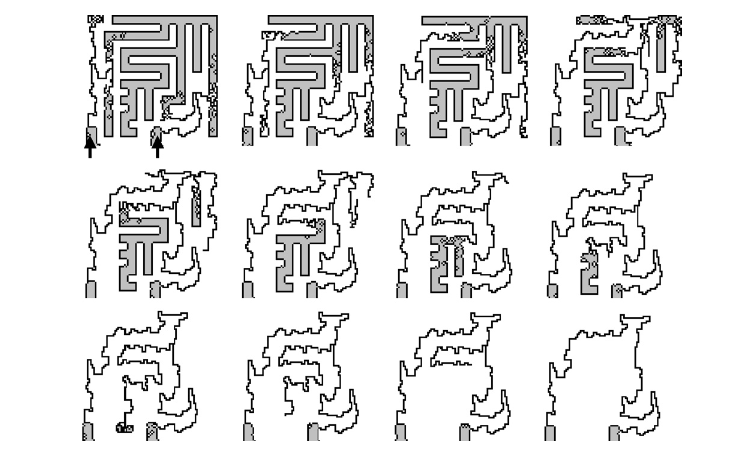
\includegraphics[width=0.7\textwidth]{./images/estado_del_arte/physarum/laberintoGunji.png}
        \caption{Aplicaci\'on del algoritmo para resolver un laberinto utilizando el modelo de \textit{Physarum polycephalum}. \cite{gunji2008}}
        \label{fig:cell_algorithm}
    \end{figure}
    \vskip 0.5cm
    Las reglas del modelo se describen en la Figura \ref{fig:cell_rules}, mostrando los diferentes 
        estados de los sitios y c\'omo interact\'uan durante las fases de desarrollo y b\'usqueda de alimento.
    \vskip 0.5cm
    % Imagen de las reglas del modelo
    \begin{figure}[h]
        \centering
        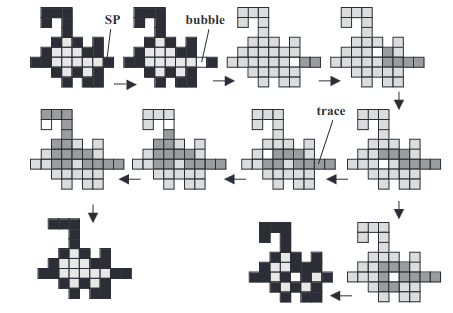
\includegraphics[width=0.7\textwidth]{./images/estado_del_arte/physarum/rGunji.png}
        \caption{Reglas del modelo de c\'elula m\'inima, mostrando los estados de los sitios y las interacciones. \cite{gunji2008}}
        \label{fig:cell_rules}
    \end{figure}
